
\section{AR Annotation using 3D sensors}
\label{sec:3D}

% =============== PREVIOUS WORK ================

% A. Nassani, H. Bai, G. Lee, and M. Billinghurst, “Tag it!: AR annotation using wearable sensors,” in SIGGRAPH ASIA 2015 Mobile Graphics and Interactive Applications on - SA '15, 2015, pp. 1–4.

% A. Nassani, H. Bai, G. Lee, and M. Billinghurst, “Extending HMD by chest-worn 3D camera for AR annotation,” in SIGGRAPH ASIA 2015 Mobile Graphics and Interactive Applications on - SA '15, 2015, no. Figure 2, pp. 1–2.

% =============== PREVIOUS WORK ================


% \subsection{abstract}

In this work we describe a wearable system that allows people to place and interact with 3D virtual tags placed around them. This uses two wearable technologies: a head-worn wearable computer (Google Glass) and a chest-worn depth sensor (Tango). The Google Glass is used to generate and display virtual information to the user, while the Tango is used to provide robust indoor position tracking for the Glass. The Tango enables spatial awareness of the surrounding world using various motion sensors including 3D depth sensing, an accelerometer and a motion tracking camera. Using these systems together allows users to create a virtual tag via voice input and then register this tag to a physical object or position in 3D space as an augmented annotation. We describe the design and implementation of the system, user feedback,  research implications, and directions for future work.  


% \subsection{Introduction}


% In our research we are interested in allowing people to place virtual tags at points or objects of interest in their physical world. Recent developments in wearable computing have made this possible by integrating sensing, interaction and display technologies into small body-worn devices. Compared with traditional mobile devices, state-of-the-art wearable devices provide novel interfaces to work with the augmented digital contents, and make the Augmented Reality (AR) applications more natural and intuitive to use. For example, the head-worn Google Glass\footnote{	http://www.google.com/glass/start/} allows people to interact using their voice and head movements while freeing their hands for other tasks. Moreover,the Tango \footnote{https://www.google.com/atap/project-tango/} offers the capability of spatial awareness through tracking the 3D position of the device using a depth-sensing camera. It provides the Visual Inertial Odometry (VIO) data that gives the user's global position and orientation in 3D space to assist them to interact with virtual objects registered in the real world in a more immersive way.

% We are interested in combining various wearable technologies to enhance the AR experience. We investigate a scenario where the user wears Glass together with the Tango mounted on their chest to create and review 3D augmented annotations indoors (see Figure\ref{system}). The process of creating AR annotations using the 3D sensor is separate from viewing AR annotation using a head-mounted display (HMD). For example, users' have to turn their body to face the AR tag during creation, however for viewing the AR tags, the user can turn their head to explore the surrounding environment, separate from where their body is facing. The benefit is that it makes the user very natural and comfortable.

% \begin{figure}[ht]
%   \centering
%   \includegraphics[width=\linewidth]{images/mgia16/sampleteaser-01}
%    \caption{AR annotation application scenario. (a) The user is wearing Google Glass on her head and a Tango device on her chest; (b) A sample indoor environment for spatial tagging; (c) The corresponding depth and VIO data from the Tango sensors; (d) The AR view through the Glass display: a virtual tag is now attached a real location on the table.}
%   \label{system}
% \end{figure}

% \subsection{Related Work}

% There have been a number of examples of AR annotation demonstration on mobile devices. For example, mobile AR browsers (e.g. Wikitude or Junaio) can overlay AR tags in the real world using  GPS and other motions sensors. While they were successful with demonstrating the concept of visualizing AR annotation, the registration of virtual objects in the real world can be inaccurate and they can only be used in outdoor large-scale environments. Mobile AR browsers usually create AR tags in advance, but recent research projects have investigated in-situ and interactive creation of AR tags. Kim et al. \cite{Kim:2011:IAS} presented an interactive method where the user stands in a fixed position to calibrate the room model with the gyroscope data. The user can then touch and annotate locations with a rectangle where virtual content, like text, image and 3D models, can be overlaid.  Langlotz et al. \cite{Langlotz:2012:OCP} developed a vision-based orientation tracking system to locate and visualize annotations with pixel accuracy on a real-time generated panorama. Both these systems assume pure rotation from the devices while the user has to stand at the same position while doing the annotation, which dramatically reduces the user experience.

% Meanwhile, a variety of AR annotation methods with wearable interfaces have been presented as well. Sixsense \cite{Mistry:2009:WWU} used a wearable gestural interface for AR annotation. It consists of a camera and a small projector mounted on a hat or coupled in a pendant. The camera tracks user hand gestures and the projector visually augments virtual content on the physical objects that the user is interacting with. However it requires planar surfaces in front of the user for accurate projection because of the lacking of a depth sensor. OmniTouch \cite{Harrison:2011:OTW} is a wearable projection system equipped with depth-sensing technology that enables interactive multi-touch applications on different surfaces. Both the depth camera and projector are rigidly mounted to a form-fitting metal frame, which is worn on the shoulders, and secured with a chest strap. This system extended the typical scenarios supported by Sixsense to  users' on-body surfaces or objects held in hands for image projection by using depth sensors. However, the system itself is still bulky and inconvenient to use because of the need to connect to a desktop computer.

Our system overcomes the limitations mentioned above by combining multiple wearable technologies through a wireless network. The system is small and light enough to comfortably wear, allowing for mobility in the physical world, and being available for annotation not only on 2D surfaces but in 3D space. For example, if the user walks closer to or away from the AR tag (e.g. 3D text or models), it will appear bigger or smaller according to the changes in the perspective view. The system combines Google Glass and Google Tango together to provide compelling wearable AR experience. Google Tango is a self-contained handheld device that contains a motion tracking camera, 3D depth sensing a nine axis accelerometer, gyroscope, compass sensors. It has a rear-facing 4MP RGB/infrared camera, a 180-degree field-of-view fisheye rear-facing camera, a 120-degree field-of-view front facing camera, and a 320 x 180 depth sensor. In contrast, Google Glass has no depth sensing capability but combines computing and display in a highly compact form factor. Connecting the two devices enables us to easily prototype future wearable AR interfaces such as what might be possible with Microsoft Hololens\footnote{https://www.microsoft.com/microsoft-hololens/en-us} or other devices.

\subsection{System Design}

The main application scenario for our prototype system is around sharing messages through creating and viewing location-based AR tags registered in a small scale physical environment. The user wearing the system walks into a room and then places AR tags at various places or on objects. The AR tag content is created by using voice input and placed where the user is looking. The AR tags can be meaningful for users, for example, reminding them of something interesting in this space, or sharing the message with other users as a collaborative tool. The system should work in an arbitrary unprepared indoor environment where no previous knowledge about the space is required. 

Traditionally AR tag tracking uses two different approaches at different  ends off the technology spectrum (see Figure\ref{fig:mgia16:spectrum}) based on the level of detailed information required. At one end there is GPS location-based tracking that can be implemented in a light weight HMD such as Glass. On the other end 3D depth sensing cameras incorporated into a hand-held device (HHD) are capable of indoor tracking and localization. The aim of this system is to combine the benefits of a light weight HMD with a self-contained mobile 3D depth tracking offering not only the outdoor GPS based tracking but also vision based indoor tracking  for AR annotation applications. 


\begin{figure}[ht]
  \centering
  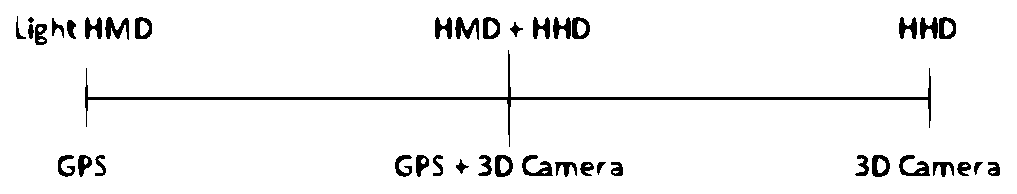
\includegraphics[width=.8\linewidth]{images/mgia16/tango_paper_continuum}
  \caption{The spectrum of AR tag tracking. A head-mounted display with GPS is ideal for outdoor tracking. Hand-held devices (3D camera) can be used for indoor tracking. Glass+Tango enables indoor AR tag tracking on light HMD.}
  \label{fig:mgia16:spectrum}
\end{figure}

\subsection{Implementation}


\begin{figure*}[t]
  \centering
  \includegraphics[width=\linewidth]{images/mgia16/workflow_diagram}
  \caption{System workflow.}
  \label{framework}
\end{figure*}


The system consists of two wearable devices a Google Glass HMD and a Google Tango chest-mounted 3D depth and sensor (see Figure\ref{framework}).

The two devices communicate with each other wirelessly. The Tango extends Glass' sensing ability by sharing the location and pose of the user as well as the tagged target position in the real world. The Glass dynamically overlays virtual tags based on the spatial information received from the Tango, and the background of the Glass display is set to black to act as an optical see through display (see Figure\ref{fig:mgia16:ui}). A white square is displayed on the Glass screen to indicate the center point at which the tango depth camera is facing. The user can initiate the wireless connection by using a three-finger touch gesture on the Glass touchpad, and the AllJoyn library  is used for networking.

Once the system starts on the Tango, it creates a reference coordinate of the surrounding environment. When the user moves, the motion sensor on the Tango will detect the body  position and rotation from the reference origin, both of which are then wirelessly transmitted to the Glass. Combing the head rotation detected by the sensors on the Glass, we can calculate the AR Viewpoint. The position of the AR viewpoint is calculated by adding a measured distance in height from Tango's position to adjust the height difference between the Glass and Tango. The orientation of the AR viewpoint mainly depends on the body's rotation but will be adjusted with the head and body pose difference, if the user turns their head towards a different direction from their chest. 

A speech recognition service is running in the background on the Glass to detect the users' voice input and convert it into text. The text will appear on the upper left corner of the display for for the users confirmation. This function is implemented as an Android service that utilizes Google API for speech recognition and so requires an internet connection. Once the user is satisfied with the recognized text, they can tap on the Glass touchpad while looking where they wish to add the AR tag by using the white square in the display. The Glass sends a request to Tango to identify the location of the AR tag in 3D space.

Combining the AR view point and the recognized text, we can convert the target position (the center point of the depth image indicated by the white square) to the global position relative to the origin. The Tango returns the global position of the AR tag to the Glass. This information is used to construct an AR tag with the speech recognized text that is overlaid on the top of the Glass camera view.

In (Figure\ref{fig:mgia16:ui}), the top left corner shows the last words captured via the voice recognition service, and a white square indicates the center position of Tango's RGB depth frame. The text in the middle of the display "Cup" is an AR tag overlaid on top of a physical cup. 
% * <eng.ala@gmail.com> 2015-06-19T10:04:56.888Z:
%
%  [Somewhere it would be good to mention the tracking accuracy and update speed – how accurate is the Tango position sensing for example]
%

\begin{figure}[ht]
  \centering
  \includegraphics[width=2.5in]{images/mgia16/WIN_20150614_204531_2}
  \caption{View through Glass display of a cup overlaid by an AR tag.}
  \label{fig:mgia16:ui}
\end{figure}


\subsection{User Study }

To evaluate our prototype, we conducted a pilot user study (see Figure\ref{fig:mgia16:scenario}) with ten participants . 4 female, 6 male ranging in age between 23 to 33 years old (\textit{SD= 4.35}). The main focus of the study was to measure the usefulness of the proposed system. Participants were asked to create three different AR tags for three different objects inside the room, with voice input, and then to walk around to observe how well the AR annotation is placed at the selected location. Participants had the freedom to assign any text to any object they wish in the test. The experiment conductor explained the tasks before the experiment and gave examples of target objects and names to use for voice input. All participants completed the tasks within 5 minutes. 

\begin{figure}[ht]
  \centering
  \includegraphics[width=3in]{images/mgia16/axis_lo}
  \caption{User study scenario}
  \label{fig:mgia16:scenario}
\end{figure}

Qualitative feedback about the system was collected from participants including how they would describe their experience using our system, what they liked and didn't like. Questions (Table \ref{table:questions}) were in four categories: (C1) Using the voice commands to create AR tag, (C2) Tap on glass touch panel to attach the AR tag, (C3)  Walk around to find AR tag stick to the original position, (C4) Overall AR tagging experience. In each category we asked the participants the following questions

\begin{table}[ht]
  \centering
	\caption{Survey questions}
    \label{table:questions}
    \begin{tabular}{r l}
    \hline
    Q1 & I found it easy to use \\ \hline
    Q2 & I found it natural to use \\ \hline
    Q3 & I found it physically challenging \\ \hline
    Q4 & I found it mentally challenging \\ \hline
    Q5 & I found it useful \\ \hline
    \end{tabular}
\end{table}

The answers were captured on a Likert scale of 1 to 7 in which 1 is "strongly disagree" and 7 is "strongly agree".

We used the Wilcoxon Signed Rank test on the results to measure significance. Based on the results, we found that participants rated significantly higher than neutral (4) on Q3 (p=.01, .009, .007 and .041) and Q4 (p=.014, .009, .007 and .01) for all categories (C1, C2, C3, C4). Q2 (p=.033) and Q5 (p=.015) were rated significantly higher for category (C3). Q1 for C4 was rated significantly higher (p=.014). (see \ref{survey_results}). The results  for other tasks were rated less significant than neutral level (4). Participants rated the task of walking around the environment was useful with average score of 5.2 out of 7 as well as being not mentally challenging with an average score of 2 out of 7. This highlights the usefulness of the system in assigning AR tags and recognizing them when they appear on their display while walking around the environment. 

In addition to the survey, we also asked participants open questions to comment on the system usability. A total of 3 out of 5 participants mentioned that they would use this system for virtual sticky notes, and they also provided some positive feedback such as "the system could be useful for finding a meeting room or a colleague's desk in an open plan area". There were also a few suggestions for improving the system, such as "allow the user to manually adjust the location of the AR tag" or "integrate with eye tracking to assist placing the AR tag within the field of view ". Participants appreciated  the concept of wirelessly connecting depth camera to a wearable HMD to enable the 3D spatial tracking.    


\begin{figure}[ht]
  \centering
  \includegraphics[width=\linewidth]{images/mgia16/user_study_results2}
  \caption{Average results of survey questions. Bars indicate standard error. *=statistically significant}
	\label{survey_results}
\end{figure}


\subsection{Discussion}

% * <eng.ala@gmail.com> 2015-06-19T10:05:25.941Z:
%
%  It would be good to add some more comments about why you got the results that you did
%
While our prototype  system demonstrates the concept of harmonizing the use of multiple wearable devices for AR visualization, there are few limitations in the current implementation of the system. It was observed that some users had difficulties with voice input as they were not native English speakers, which made the participants use several attempts before the intended word was correctly recognized.  

The current system tracks the 3D environment relative to the starting position, which requires the users to start the system at the same position and orientation in each test trail to keep the annotation in place between uses for sharing. This could be overcome in the future by storing the reconstructed 3D map of the environment and reusing it instead of generating it from scratch every time. 

\subsection{Future Application Scenarios}

Many implementation scenarios could benefit from combining a light head-mounted display with a chest worn 3D depth camera,  such as 1) Navigation, 2) Remote collaboration and 3) Social sharing. In this section we describe each of these in more detail.

Navigation is a scenario where this system can be useful. The user could navigate in an outdoor environment using GPS on Glass or similar smart glass display. Google Glass, being an unobtrusive head-mounted display, allows for hands-free navigation. However when the user enters a building, the GPS stops working and the system switches to indoor navigation using the 3D depth camera of the Google Tango device. Combining two devices enables seamless transition during a navigation experience. For example, a person could be shopping to find a particular item and use outdoor GPS tracking to guide them to the store. Once inside the store the Tango depth sensing hardware can help with navigating to find the particular product on the shelf.

Remote collaboration is another scenario where this application could be useful. A local user could transmit reconstructed 3D geometry of the environment using the Tango device to the remote user. The remote user will then have a more detailed view of the environment comparing to 2D sharing such as with a video stream. With the 3D geometry of the environment, the remote user can view the scene from different angles that helps provide better understanding of the surroundings of the local user. Placing AR tags in a 3D environment helps maintain the location of the AR tag especially when the viewing perspective is changed to the point from when it was original recorded

An additional use of the system could be in a social sharing experience where multiple users of the system could collaborate to add, edit and manipulate AR tags in the shared environment. 
% * <eng.ala@gmail.com> 2015-06-19T10:02:27.344Z:
%
%  put more information
%

\subsection{Summary}

This section presented a wearable AR system combining tracking technologies to provide a compelling indoor AR experience for spatial annotation application. By wearing the system, users can create virtual tags with text content generated by voice input and place it where they are looking at. The virtual tags can be visualized in place as a reminder for the users.  

Different scenarios can be implemented and tested based on the prototype with multi wearable devices. There are also a number of ways this research could be extended. In the future, we would like to further develop our efforts in designing interaction scenarios for our system, such as wearable gaming or collaboration. We also plan to develop the system further to expand the use of chest worn device for various interaction techniques (e.g. gesture recognition).
